\subsection{Web Subsystem}
\label{sec:web_subsystem}
The web subsystem will be split into several distinct parts to achieve several goals. First and foremost, the web will communicate over TCP with the MCU to get data, process the data and send commands back to the MCU. Secondly, there will need to be a database in order to log data and be able to support multiple of these garden beds in a scaled solution. Third, there needs to be a user interface that allows the user to set settings and read the data about their garden bed(s). Lastly, the web component of this project will communicate using HTTP requests with a weather service to get upcoming weather such as rain, sunlight, and freeze warnings in order to help the user with maintaining their plant bed.


The block diagram below shows a high level overview of flow of data between different sources. The microcontroller and web component share a two way interface to transmit controller data to the web and commands back to the MCU. Refer to the MCU subsection for more details on the commands. Part of the this component will be a way to process the data received from the weather service and the MCU to serve it to the UI and thus the user. 
\begin{figure}[H]
    \caption{Web component block diagram}
    \centering
    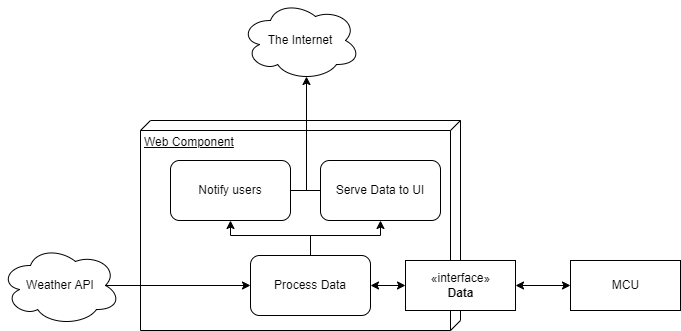
\includegraphics[width=\textwidth]{images/WebBlock.png}
\end{figure}
Section \ref{sec:web-tech} has information on the technologies in the stack while the following sections will go into more detail about how these choices will be used in order to achieve the goals outlined above. These choices are a React frontend as it is a technology that the team is familiar with and has good support and allows for an event-driven UI as would be useful to serve the polling data collection of the backend. Express will be used as a middleware and routing layer for the user interface to the server backend. This choice was made again to keep the language in JavaScript and the vastness of suppport on the platform. Express also supports Socket.js which will be necessary for communicating over TCP with the microcontroller. MySQL will be used as a relational database as the data is relational. SQL databases also typically serve data-driven applications better over service-driven.
\subsubsection{Server Backend}
As mentioned above, the backend will consist of two parts, a MySQL database as this is a free option and serves the purposes well especially for logging data, as well as an Express backend which will serve all the API endpoints for the user interface as well as a serve to create TCP connections with the microcontroller.
\paragraph{Communication}
This section will cover how we plan on implementing communications with the microcontroller. As covered in \ref{sec:controller_subsystem} these two systems will communicate over TCP. The means of implementing this will be through sockets. This backend will serve as a server to make connections to. Through the use of the Socket.io library, it will be nearly superficial to create this connection and read raw data and process it. Once data is received will be stored in the database for computation.
\paragraph{Database}
The database will be relational. Relating a plant bed and its current state to the logs of data stored within the database as well. The way this will be implemented is there will be a table, \verb|garden_bed| which will store a garden bed and the client socket information. From this point, the ID of the \verb|garden_bed| will be used in a lookup in other tables such as \verb|data_solar| or \verb|data_soil| to be able to present this data to the user in the UI upon request. These data tables will have a timestamp of their creation to be able to lookup the most recent data and retrieve those items and also to create a log and graphs if we so chose. Figure \ref{fig:erd} has some details on the type of data and where it can be found within the database given the design above.
\begin{figure}[H]
    \caption{Entity relationship diagram}
    \centering
    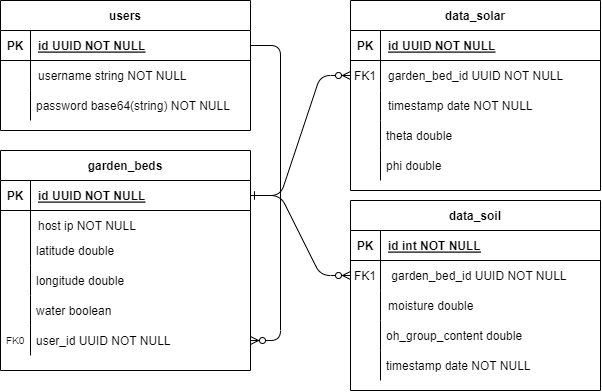
\includegraphics[width=\textwidth]{images/EntityRelation.png}
    \label{fig:erd}
\end{figure}
Another option for the organization of the database is to create a table for each plant bed, which for this project would only be one, that holds all the data and logs regarding to that plant bed. This solution is slightly harder to implement. It is harder to implement because ORMs (Object-Relational Mapping) do not like the dynamic nature of tables. ORMs know the schema of a database table per the name, and when the database becomes highly dynamic in this architecture, the ORM typically requires more work to setup. For more detail on ORMs refer to the technology section of this document.
\paragraph{Data Processing}
All data will be processed on the EC2 instance within the server. Using some heuristic methods and research into peak conditions for different plant types, the server will be able to determine different actions to be made on the plant bed in order to promote growth.
\paragraph{Accounts and Plant Bed Linkages}
Each user account will be linked with potentially multiple plant beds through the database designed above. The backend will validate user logins to endpoints using JWTs in cookies in order to validate each user that logs in.
\paragraph{API Endpoint Design}
Representational State Transfer (REST) is a paradigm that indicates a certain API is platform agnostic thus allowing for any number of clients to call the API so long as they follow the standards that are implemented. REST is typically implemented through HTTP requests, this is the case for our project as well. HTTP comes fully packaged with various methods of calling different URIs (unique resource identifier). The best way to represent this is that a top-level domain refers to the server while appendages to the domain denote the resource and the verb. For example, \verb|http://autogardenbed.com/garden|, is the location of the garden resource. From there we can use HTTP methods to instruct the server on what action to take. The most common operations are POST, GET, PUT, DELETE which corresponds to create, read, update, and delete. Our API will be no different.

The URIs will follow the convention of \verb|.../[noun]/[verb]/{identifier}|. The ``noun'' refers to the type of object that the request will interact with. In our case this should be something like ``garden'' or ``data''. Verbs will be used rarely but a situation that might arise is where the user wants to send a command to their garden bed. This will be accomplished through the verb portion of the URI. \autoref{table:uris} gives a high level overview of the URIs, the associated methods and what they will accomplish.
\begin{table}[H]
    \centering
    \begin{tabular}{c|p{2cm}|p{6cm}}
        \hline
        \textbf{URI} & \textbf{HTTP Method} & \textbf{Function} \\
        \hline
        \multirow{4}{*}{\texttt{.../user}} & POST & Create a new user \\\cline{2-3}
                                           & GET & Get a user's information such as a list of associated garden beds\\\cline{2-3}
                                           & PUT & Update user information such a password \\\cline{2-3}
                                           & DELETE & Delete user account \\\hline
        \texttt{.../user/auth} & POST & Takes user credentials and validates against database; returns a JWT for validation in other endpoints \\
        \hline
        \multirow{4}{*}{\texttt{.../garden}} & POST & Creates a new garden bed \\\cline{2-3}
                          & GET & Get data on a garden bed, join garden bed info with data  \\\cline{2-3}
                          & PUT & Update garden bed information, such as IP, location, etc. \\\cline{2-3}
                          & DELETE & Delete the garden bed from the database and ensure no records are orphaned \\\hline
        \texttt{.../garden/\{garden\_id\}/command} & POST & Sends the command specified by the request object to the garden bed \\
        \hline
    \end{tabular}
    \caption{URI table}
    \label{table:uris}
\end{table}
\subsubsection{User Interface}
The below hex values were selected using a color picking service that guarantees a palette that is useable for users who might be colorblind.
\begin{figure}[H]
    \caption{Color palette}
    \centering
    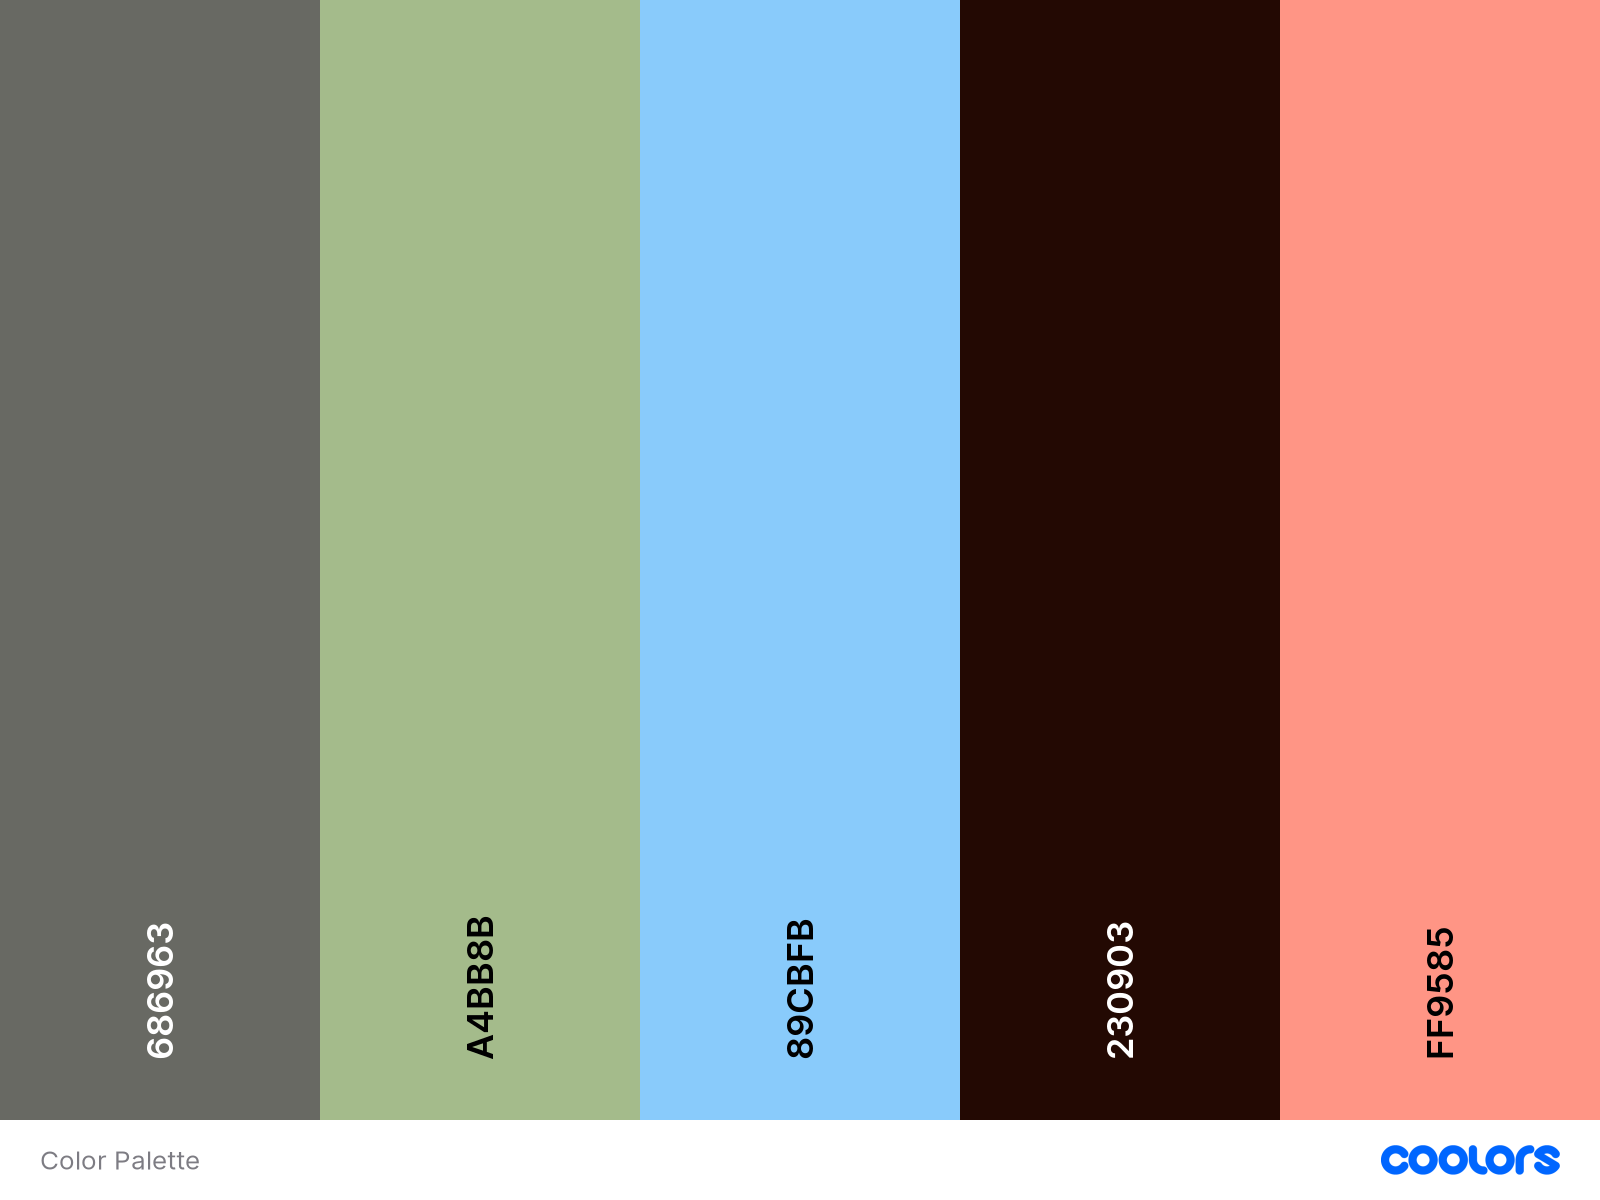
\includegraphics[width=\textwidth]{images/Color Palette.png}
    \label{fig:color_palette}
\end{figure}
For user experience, catering to colorblindness is important. From left to right the purpose of each color is: component color, emphasis, highlight, background color, error.

To design the user interface we will be using Figma. Figma offers some prototyping and features in order to quickly build a user interface. In conjunctions with React as a framework and CSS, putting everything together should be relatively trivial.